% Test: insbox (v2.2)
% \InsertBoxR{n}{box}[correction] — CAUTION: [correction] is optional,
% so the NEXT token after } will be consumed as [corr] if it starts with [.
% Use {} or \relax to prevent this.
\documentclass[11pt,a4paper]{article}
\usepackage[utf8]{inputenc}
\usepackage{graphicx}
\usepackage{lipsum}

\makeatletter
\input insbox
\makeatother

\title{insbox Test}
\author{Programmer Agent}
\date{2026-05-15}

\begin{document}
\maketitle

\section{Test 1: \InsertBoxR (right)}

\InsertBoxR{0}{%
  \fbox{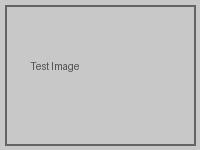
\includegraphics[width=0.28\textwidth]{test-image.png}}%
}{}
\lipsum[1-3]

\section{Test 2: \InsertBoxL (left)}

\InsertBoxL{2}{%
  \fbox{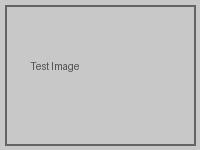
\includegraphics[width=0.25\textwidth]{test-image.png}}%
}{}
\lipsum[4-5]

\section{Test 3: \InsertBoxR near page break}

\lipsum[6-7]

\InsertBoxR{0}{%
  \fbox{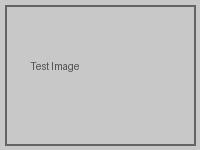
\includegraphics[width=0.28\textwidth]{test-image.png}}%
}{}
\lipsum[8-9]

\end{document}
